
\documentclass[25pt, a0paper, portrait, margin=0mm, innermargin=15mm,
blockverticalspace=15mm, colspace=15mm, subcolspace=8mm]{tikzposter} 
\usepackage{xcolor}
\usepackage{graphicx}
\usepackage{enumitem} % For custom lists
\usepackage{tikz}
\usepackage[font=small,labelfont=bf]{caption}
\usepackage{lipsum}

\tikzposterlatexaffectionproofoff



%\title{\parbox{\linewidth}{\centering \fontsize{72}{70}\selectfont Measuring changes in the speed of %transcription elongation and intron splicing}}


%\institute{\parbox{\linewidth}{\centering \fontsize{38}{48}\selectfont University of Cologne \\ % Cologne Excellence Cluster on Cellular Stress Responses in Aging-Associated Diseases (CECAD)}}

% \author{\parbox{\linewidth}{\centering \fontsize{42}{42}\selectfont Jakub Koubele, Andreas Beyer}}

\newcommand{\affil}[1]{\textsuperscript{#1}}

\title{\parbox{\linewidth}{\centering
		\fontsize{72}{70}\selectfont
		Measuring changes in the speed of transcription elongation and intron splicing
}}

\author{\parbox{\linewidth}{\centering
		\fontsize{42}{44}\selectfont
		Jakub Koubele\affil{1,2} \quad Andreas Beyer\affil{1,2}
}}

\institute{\parbox{\linewidth}{\centering
		\fontsize{32}{36}\selectfont
		\affil{1} University of Cologne\\
		\affil{2} CECAD — Cologne Excellence Cluster on Cellular Stress Responses in Aging-Associated Diseases
		% (optional email line)
		% \\[3mm]\fontsize{28}{32}\selectfont \texttt{jakub.koubele@uni-koeln.de}
}}

% Define custom colors using HTML-style hexadecimal notation
\definecolor{blue1}{HTML}{005BA6}  % #005BA6 as custom blue
\definecolor{blue2}{HTML}{005176} % Example: gold yellow
\definecolor{weakBlue}{HTML}{E5EEF6}
\definecolor{customOrange}{HTML}{FFA500} % Example: orange

\definecolorstyle{CecadColorStyle} {
	\definecolor{color1}{named}{blue1}
	\definecolor{color2}{named}{orange}
	\definecolor{color3}{named}{blue2}
	\definecolor{color4}{named}{white}
}{
	% Background Colors
	\colorlet{backgroundcolor}{color4}
	\colorlet{framecolor}{color3}
	% Title Colors
	\colorlet{titlefgcolor}{white}
	\colorlet{titlebgcolor}{color1}
	\colorlet{titleframecolor}{color2}
	% Block Colors
	\colorlet{blocktitlebgcolor}{color3}
	\colorlet{blocktitlefgcolor}{white}
	\colorlet{blockbodybgcolor}{white}
	\colorlet{blockbodyfgcolor}{black}
	% Innerblock Colors
	\colorlet{innerblocktitlebgcolor}{white}
	\colorlet{innerblocktitlefgcolor}{black}
	\colorlet{innerblockbodybgcolor}{color3!30!white}
	\colorlet{innerblockbodyfgcolor}{black} % Corrected line
	% Note colors
	\colorlet{notefgcolor}{black}
	\colorlet{notebgcolor}{color2!50!white}
	\colorlet{noteframecolor}{color2}
}

\usecolorstyle{CecadColorStyle}

% Define reference block style
\defineblockstyle{referenceblock}{
	draw=white, % Border color
	line width=0pt, % Border thickness
	rounded corners=1mm, % Rounded corners
	inner sep=5pt, % Inner separation
	fill=white, % Background color
	font=\small % Font size
}{}


\usetitlestyle{Filled}
\begin{document}
	\maketitle % See Section 4.1	
	 %\node[anchor=west, xshift=72cm, yshift=-10cm] at (TP@title.west) % 
  %{
\includegraphics[width=8cm]{figures/uni_logo.png}};
		
	\begin{columns} % See Section 4.4
		\column{0.5} % See Section 4.4
		
		\block{Introduction}{
			\begin{itemize}
				\item \lipsum[1][1-3]
		
		
			\item \lipsum[1][4-6]
		\end{itemize}
		}
		
		\block{Method}{
		\begin{itemize}
				\item \lipsum[1][7-9]		
				
		\end{itemize}
		
		\begin{center}
			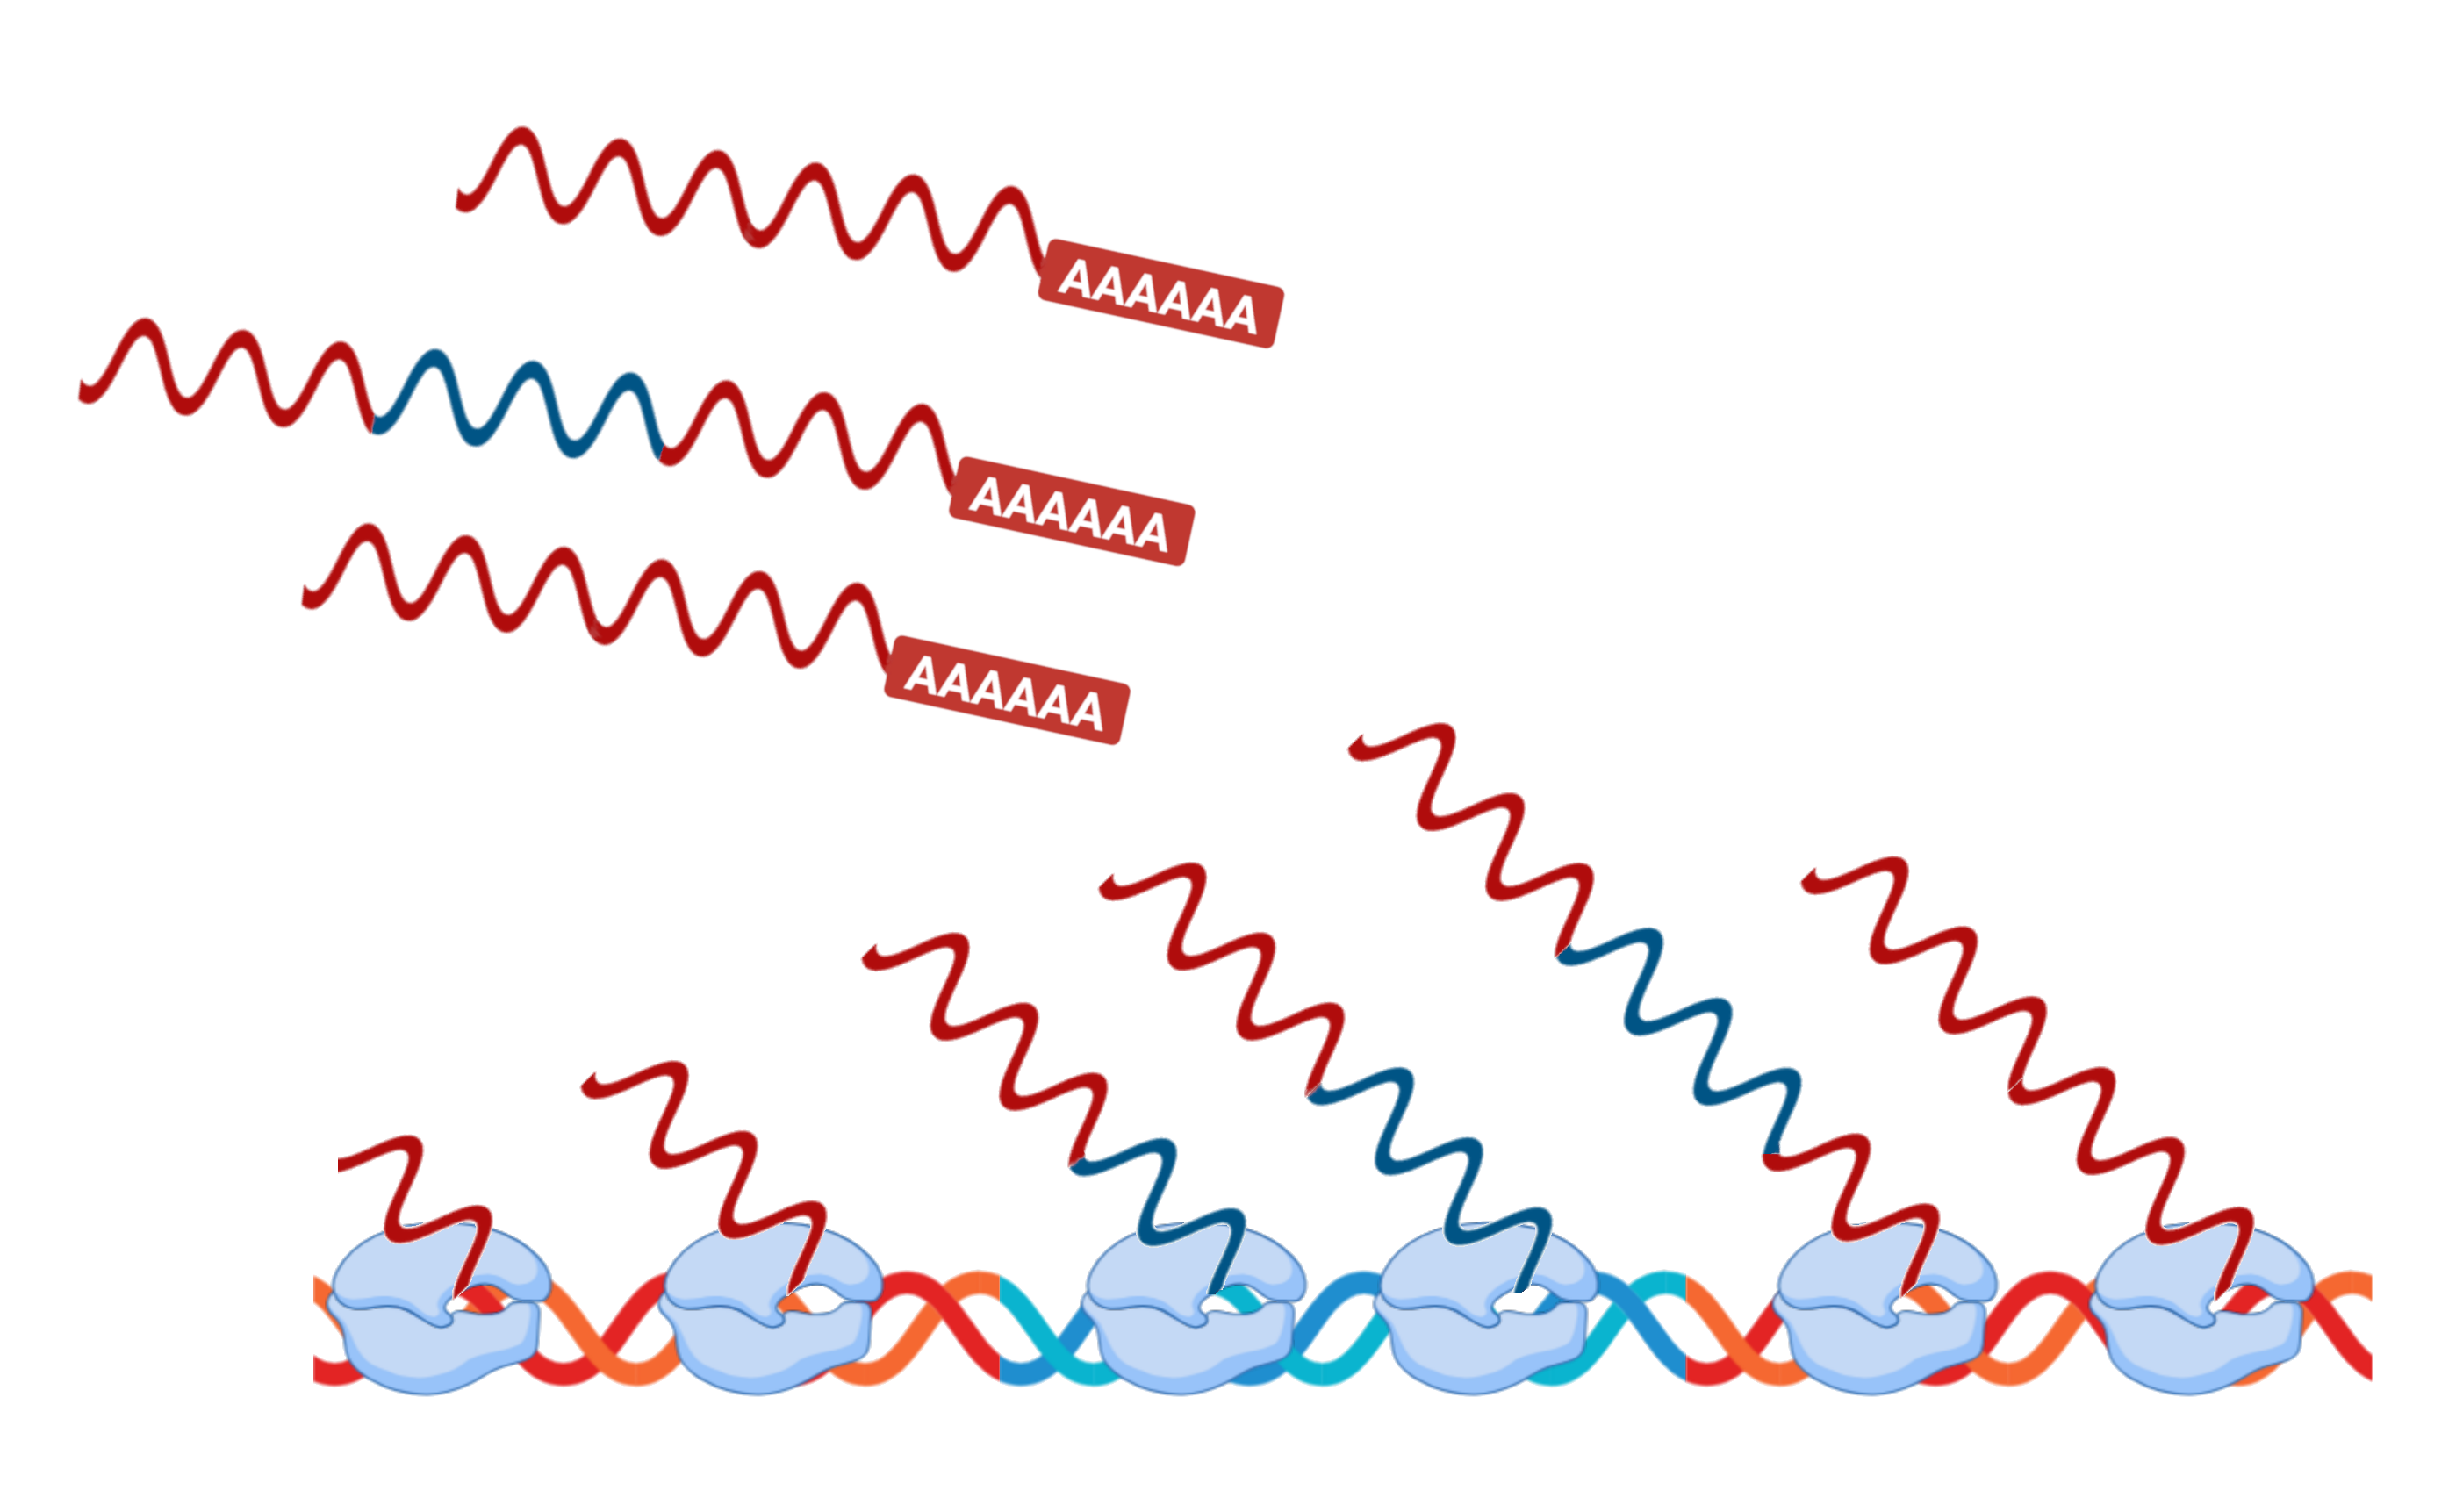
\includegraphics[width=0.7\linewidth]{figures/total_rna_with_bg.png}\\[1ex]
			\small\textbf{Figure 1.} Total RNA-seq
		\end{center}
		
		
		
		
		
		\begin{itemize}
			\item \lipsum[1][10-12]
			
		\end{itemize}
		
		\begin{center}
			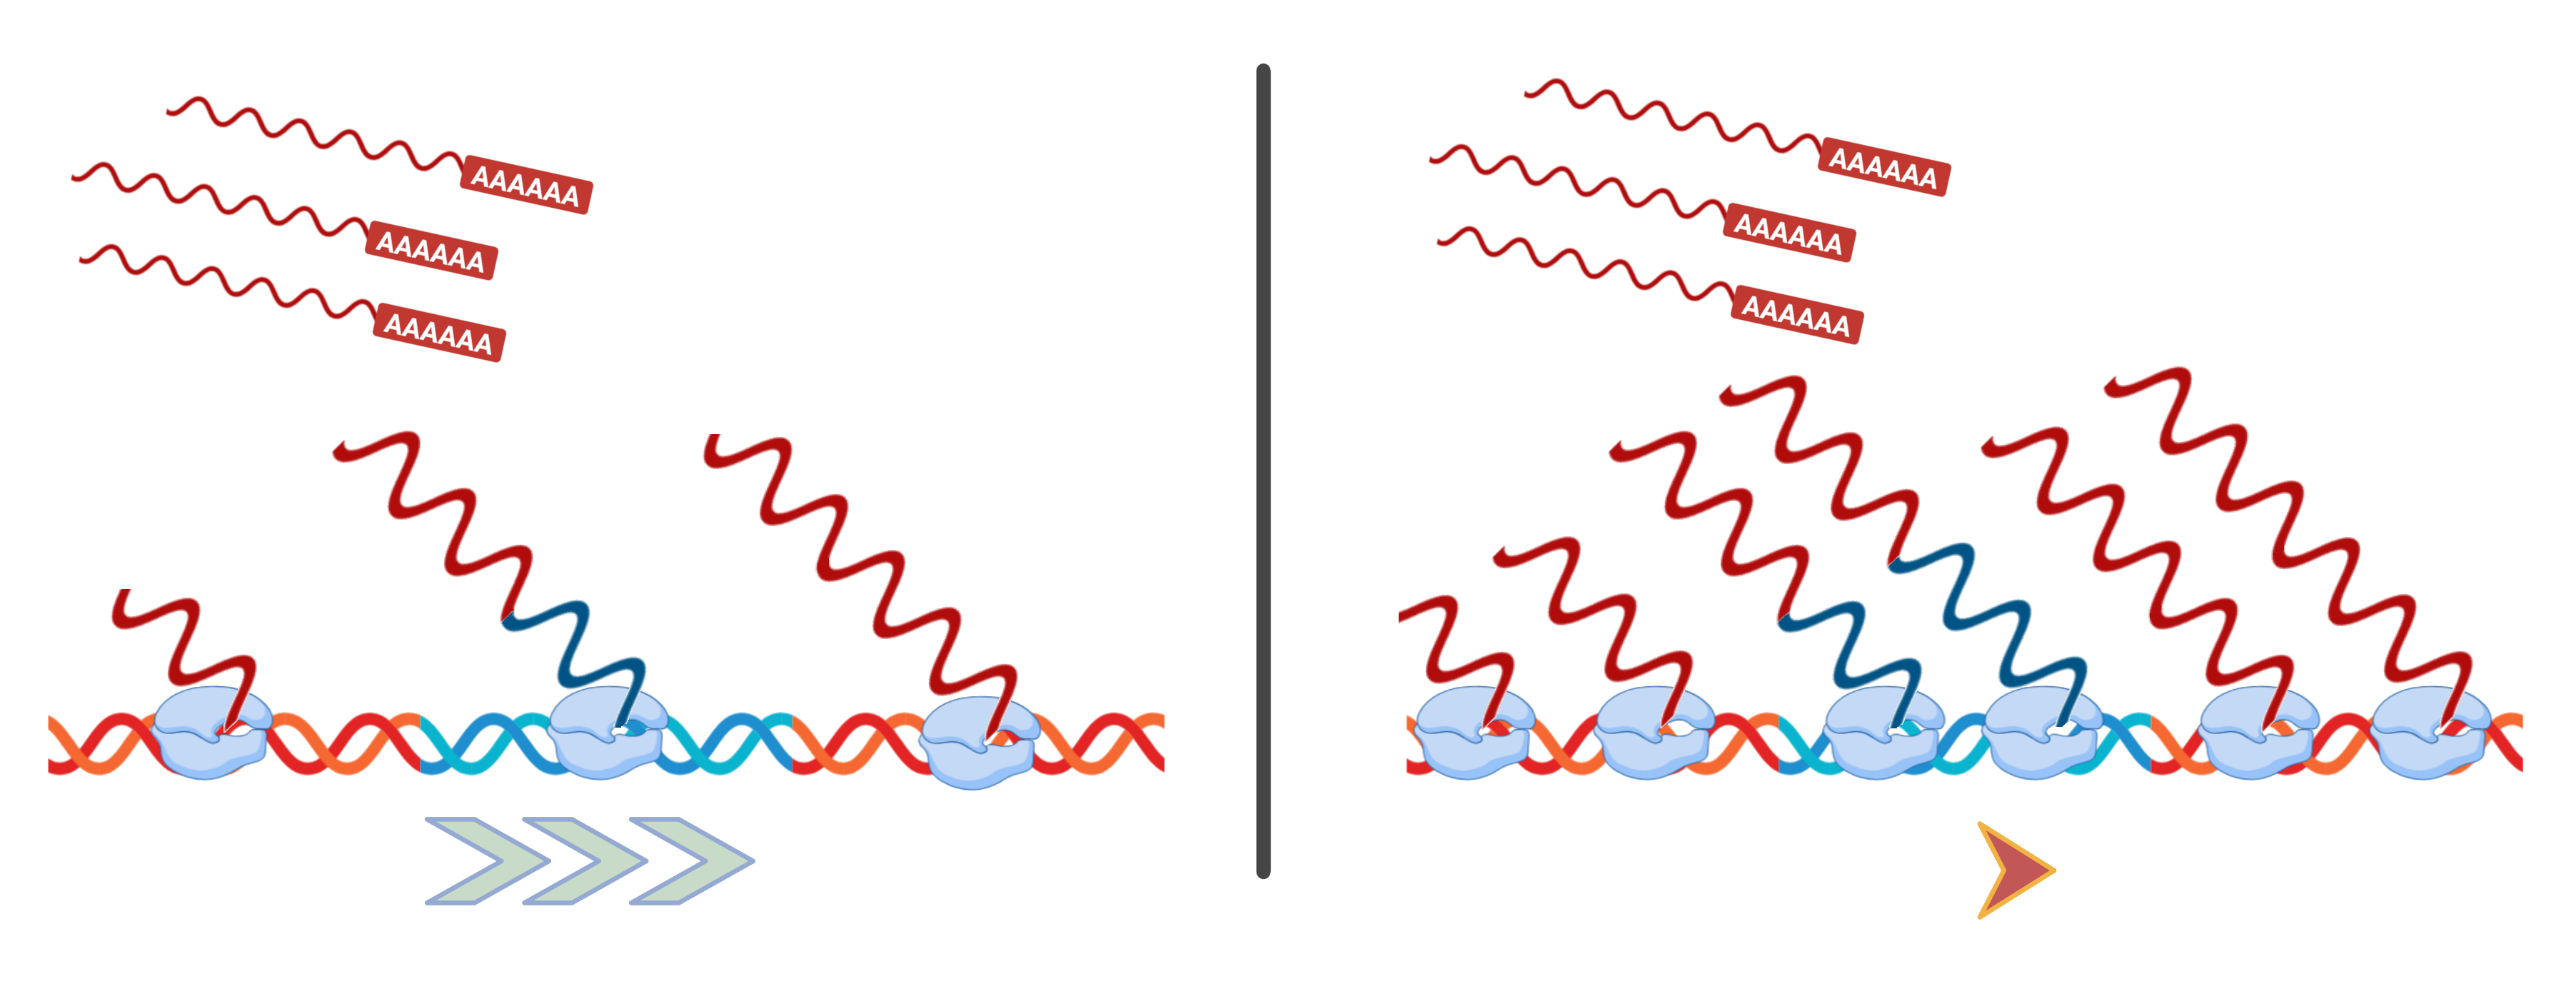
\includegraphics[width=0.7\linewidth]{figures/pol_ii_speed_figure.png}\\[1ex]
			\small\textbf{Figure 1.} Total RNA-seq
		\end{center}
		
		\begin{itemize}
			\item \lipsum[1][13-15]
			
		\end{itemize}
		
		\begin{center}
			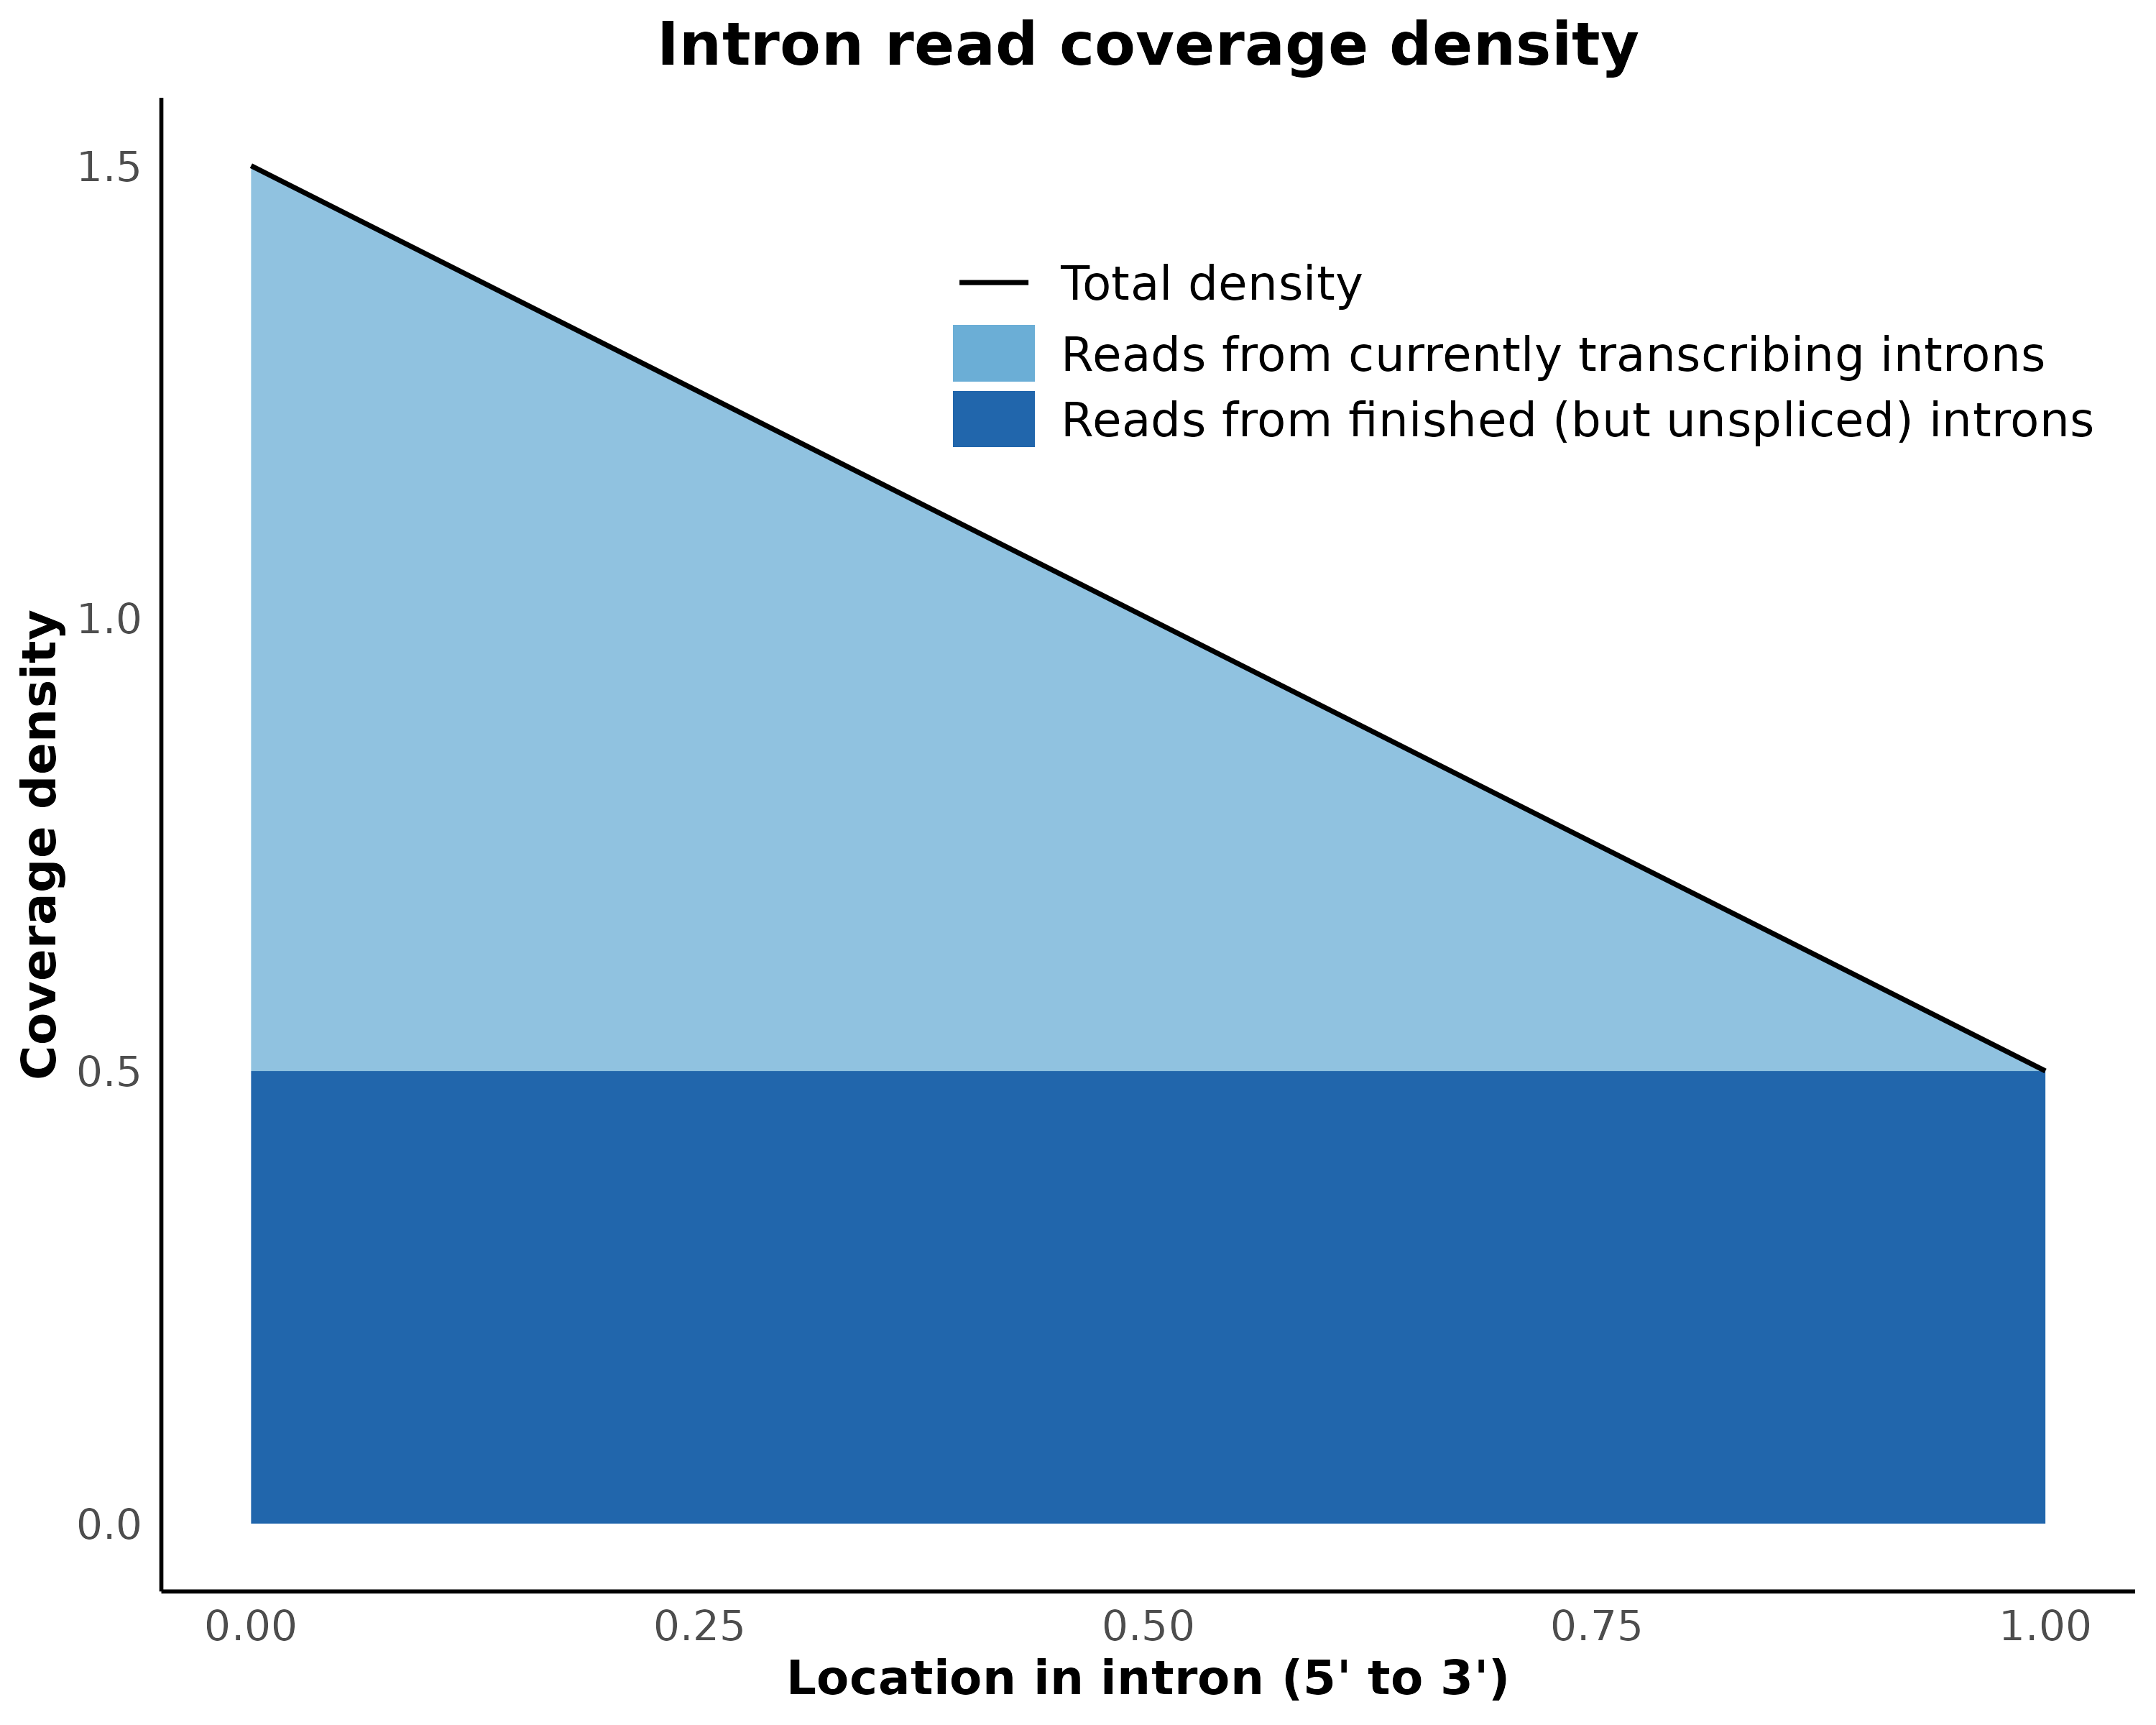
\includegraphics[width=0.7\linewidth]{figures/density_plot.png}\\[1ex]
			\small\textbf{Figure 1.} Total RNA-seq
		\end{center}
		
		
		
		}
		\column{0.5}
			\block{Results}{\begin{itemize}
					\item \textbf{Lorem Ipsum...}: 
				
				
					
			\end{itemize}
		}
		\block{Discussion}{
		\begin{itemize}
			\item Lorem Ipsum...
		\end{itemize}
	}
		
		\colorlet{blocktitlebgcolor}{weakBlue}
		\colorlet{blocktitlefgcolor}{black}
		\block{References and Acknowledgment}{
			\begin{itemize}
				\item Lorem Ipsum references
				\item Illustrations were created using BioRender.com. The poster was created using tikzposter.		
			\end{itemize}
			
	}		
	\end{columns}



% --- Footer logos as a full-width block (no overlay, no tikzpicture) ---


{
	% optional: make this block look like a footer bar
	\colorlet{blocktitlebgcolor}{white}
	\colorlet{blocktitlefgcolor}{white}
	\colorlet{blockbodybgcolor}{white}
	\colorlet{blockbodyfgcolor}{blue2}
	\block{}{% empty title -> just a body area spanning full width
		\centering
		\rule{0.94\textwidth}{0.4pt}
		\vspace{5mm}
		
		
\includegraphics[height=30mm]{figures/cecad_logo.png}\hspace{150mm}%
		
\includegraphics[height=30mm]{figures/crc_1678_transparent.png}\hspace{150mm}%
		
\includegraphics[height=30mm]{figures/uni_logo_2.png}%
		
		\vspace{5mm}		
		\vspace{2mm}
	}
}






\end{document}